%-*- mode: latex; fill-column: 70 -*-
% ex: set sts=4 ts=4 sw=4 et tw=70:
%&pdflatex

\documentclass[letterpaper,landscape]{report}
\usepackage[landscape,margin=0.5cm]{geometry}
\usepackage{color}
\usepackage{flowfram}
%\usepackage{booktabs}           % for rules in tables
\usepackage{tabularx}           % for column-width tables
\usepackage[table]{xcolor}      % color control

\usepackage[colorlinks]{hyperref}

\usepackage{multicol}
\usepackage{wrapfig}
%\setlength{\columnseprule}{1pt} % for visible divider
\setlength{\columnsep}{1cm}

\newcommand{\phttp}[1]{\href{http://#1}{#1}}
\newcommand{\ie}[0]{\emph{i.e.},\ }
\newcommand{\eg}[0]{\emph{e.g.},\ }
\newcommand{\etc}[0]{\emph{etc.}}

\usepackage{tikz}
\usetikzlibrary{calc}

\usepackage{graphicx}
\graphicspath{
 {../}
 {../pics/}
 {../datalad.org/src/content/pics/}
 {../artwork/pics/}
}

\usepackage{enumitem}           % useful for control of listings
\usepackage[compact,raggedright]{titlesec}
\usepackage{comment}

\newcommand{\epigraph}[3]{\textit{#1}\linebreak \vspace{-1.5em} \begin{flushright}\hspace{5em}\ --\ #2\linebreak\small{#3} \end{flushright}}

\pagestyle{empty}
\parindent=0pt

% Attempts to change bg color of *section headings
%\definecolor{secbgcol}{rgb}{0.9, 0.85, 0.85}
%\titleformat{\section}
%{\color{red}\normalfont\Large\bfseries}{\ndsection}{1em}{}
%\titleformat{\subsection}
%{\color{red}\normalfont\large\bfseries}{\begin{flushright}\hfill\thesubsection
%  \end{flushright}}{1em}{}
%
%\usepackage{pstricks}

% To create tables within multicols
\makeatletter
\newenvironment{ndtable}
  {\def\@captype{table}}
  {}


\newcommand{\ndheading}[3]{%
\vspace{0.5em}
\begin{ndtable}%
\rowcolors[\hline]{1}{#2}{} \arrayrulecolor{#3}
\begin{tabularx}{\columnwidth}{>{\centering\arraybackslash}X}\vspace{-.5em}\normalfont\large\bfseries
  #1\vspace{0.05em}\\\end{tabularx}
\end{ndtable}
\vspace{-.5em}
}

\definecolor{secfgcol}{RGB}{215, 6, 83}
\definecolor{secbgcol}{RGB}{255, 241, 248}
\newcommand{\ndsection}[1]{\ndheading{#1}{secbgcol}{secfgcol}}
\newcommand{\ndsubsection}[1]{\ndheading{#1}{secbgcol}{secfgcol}}


\begin{document}

\vspace{-1.5em}
%%
%% DEBIAN
%%
\begin{multicols}{3}    % 3 columns

% TODO: Most probably git-annex will just get 1-2 columns on the 2nd page

\begin{center}
\noindent

\includegraphics[width=0.5\columnwidth]{borrowed/git-annex-logo}

\url{http://git-annex.branchable.com}

% \hrule
\end{center}
\vspace{-1em}

\ndsection{git-annex}

is a distributed version control system for large files developed by
Joey Hess.  git-annex enriches regular \href{http://git-scm.com}{git}
repositories with meta-information and facilities for retrieving
and/or sending data from/to remote locations.  Actual data itself
is not directly committed to git, making git-annex repositories
lightweight and easily manageable, while still providing access to
all data upon request.

\ndsubsection{git-annex features}

\begin{description}[nolistsep,leftmargin=1pc,style=nextline]

\item[Data versioning] Every file is identified by its checksum (\eg\
  SHA256), thus guaranteeing unambiguous versioning

\item[Special remotes] Besides accessing data from other git remotes
  (\eg via ssh), data can be offloaded to the cloud (\eg\ Amazon S3
  and Glacier), or just some remote computer (via ssh or rsync)

\item[Association with web origins] Every file can have a list of
  URLs from which it can be downloaded

\item[Encryption] Data can be uploaded to remotes encrypted,
  guaranteeing privacy even when offloading sensitive data

\item[Synchronization] \emph{git-annex assistant} provides
  Dropbox-like operation: keep your data files in sync, or
  automatically offloaded, backed-up, \etc\  across multiple hosts

\item[Semi-compatible with GitHub] As a git-annex repository is just
  a git repository, it can be pushed to GitHub.  The content of data
  files, however, need to be stored in some \emph{Special remote}
  or have associated download URLs
\end{description}

\columnbreak
%\ndsubsection{git-annex use-cases}

\ndsubsection{git-annex 101}

Just learn few new commands in addition to stock \emph{git}.
\url{https://git-annex.branchable.com/walkthrough}\\
provides more details and examples

\begin{description}[nolistsep,leftmargin=1pc,style=nextline]
\item[\texttt{git init;  git annex init "repo name"}]
Initialize both git and git-annex
\item[\texttt{git annex add my\_cool\_big\_file}]
Add file(s) under control of git-annex % (they become symlinks)
\item[\texttt{git commit -a -m "message"}]
Commit as you usually do with git
\item[\texttt{git annex move my\_cool\_big\_file --to usbdrive}]
Offload the file to a repository you named ``usbdrive''
\item[\texttt{git annex whereis my\_cool\_big\_file}]
Check where file is available from
\item[\texttt{git annex get my\_cool\_big\_file}]
Fetch file back to the local repository
\end{description}

\ndsubsection{Neuroimaging datasets to play with}

We have made some datasets already available as git-annex
repositories, so \texttt{git clone ...}

\begin{description}[nolistsep,leftmargin=1pc,style=nextline]
\item[\texttt{http://psydata.ovgu.de/forrest\_gump/.git/}] Unique 7T MRI,
  fMRI, DTI dataset acquired during rich auditory stimulation. See\\
  \url{http://studyforrest.org} for more information
\item[\texttt{git://github.com/datalad/nih--videocast}] git-annex
  ``mirror'' of \url{http://videocast.nih.gov}, created and updated by
  \texttt{datalad crawl}
\item[\texttt{http://data.pymvpa.org/datasets/haxby2001/.git/}]
  Seminal work by Haxby et al. (2001) for testing and demonstrating MVPA
  techniques
\end{description}

\ndsubsection{How to install git-annex}

\texttt{apt-get install git-annex}

See \url{https://git-annex.branchable.com/install} for more (OS X,
Windows, Linux, Android)

\ndsubsection{How to get support}

\begin{description}[nolistsep,leftmargin=1pc,style=nextline]
\item[On Debian systems]
 \texttt{reportbug git-annex}
\item[Community support]
  \url{http://git-annex.branchable.com/bugs}
\item[IRC] \#git-annex at OFTC network
\end{description}

\columnbreak

%\ndsubsection{Acknowledgements}

%\section*{DataLad}
\begin{center}
\includegraphics[width=0.5\columnwidth,trim=0 27 0 0,clip]{datalad-logo2}\\
\url{http://datalad.org}
\end{center}

\ndsection{DataLad}

aims to simplify and thus facilitate delivery and sharing of
scientific data by establishing a federated data distribution.
While initially aiming to deliver public neuroimaging datasets,
DataLad will be easy to adopt more neuroscience data or other fields
of endeavor.

\ndsubsection{DataLad FAQ}
\begin{description}[nolistsep,leftmargin=1pc,style=nextline]
\item[Federated?] It is impractical to distribute data through
  \emph{classical} distribution mechanisms, where
  content is contained within packages available from the central
  location (or its mirrors).  DataLad will only collect, unify,
  monitor, and expose through convenient interfaces data available
  across a wide range of data providers
% -- data sharing initiatives,  curated collections, etc.

\item[Distributed?] DataLad uses distributed version control
  \href{http://git-scm.com}{Git} and built on top of it
  \href{http://git-annex.branchable.com}{Git-annex} for data
  logistics.  Git-annex enables \emph{distributed} operation where
  clones of the datasets could be made available across multiple sites
  and media without loosing track of data and meta-information (such
  as versioning)

\end{description}

\def\blank{\hspace{0em}\vspace{-1em}}
%\columnbreak

\ndsubsection{Planned dataset coverage}
\begin{description}[nolistsep,leftmargin=1pc,style=nextline]
\item[\phttp{OpenfMRI.org}] curated fMRI (and EEG) datasets
\item[\phttp{HumanConnectome.org}] anatomical, functional,
  diffusion MRI data from 1,200 subjects
\item[\phttp{CRCNS.org}] curated electrophysiological and neuroimaging
  datasets
\item[\href{http://fcon\_1000.projects.nitrc.org}{INDI}] a collation of various datasets and initiatives (functional
  connectome, \etc)
\end{description}

\end{multicols}


\pagebreak
\begin{tikzpicture}[remember picture,overlay]
  \node[anchor=south west,inner sep=0pt] at ($(current page.south west)+(7mm,5mm)$) {
     %\includegraphics{imgfile}
     %\includegraphics[width=0.4\linewidth]{datalad-openfmri-demo_sw.png}
     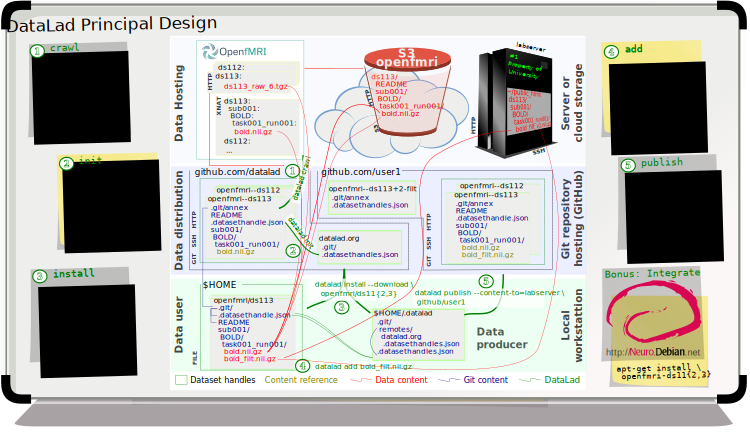
\includegraphics[width=0.65\linewidth]{datalad-whiteboard.png}
  };
\end{tikzpicture}
\vspace{-2.5em}

%%
%% DataLad
%%
\begin{multicols}{3}    % 3 columns

\ndsubsection{Planned integration}

We will expose and interface to the datasets available from

\begin{description}[nolistsep,leftmargin=1pc,style=nextline]
\item[\href{http://xnat.org}{XNAT}] widely used imaging informatics
  platform used by \phttp{HumanConnectome.org},
  \href{http://nitrc.org/ir}{NITRC-IR},
  \href{http://openfmri.org}{OpenfMRI} and others
\item[\href{http://coins.mrn.org}{COINS}] web-based neuroimaging and
  neuropsychology software suite hosting many neuroimaging datasets
\item[\href{http://academictorrents.com}{Academic Torrents}]
  collection of academic datasets delivered as
  \href{http://en.wikipedia.org/wiki/BitTorrent}{Torrents}
\item[\href{http://neuro.debian.net}{NeuroDebian}] Through the joint
  venture with the \href{http://neuro.debian.net}{NeuroDebian}
  project, DataLad will also expose itself as a
  \href{http://www.debian.org}{Debian} APT repository, making it
  possible to \emph{install} and \emph{upgrade} datasets using
  conventional tools such as \texttt{apt} and \texttt{aptitude}.
  Data \emph{installation} would become as easy as software installation.
\end{description}


%\ndsubsection{Principal Schema}
\vspace{27em}

{\tiny \color{white}.}
\columnbreak

\ndsubsection{How could you help \emph{both of us}?}

Sharing scientific data is not yet as easy as it could and should be.
Adhering to the following guidelines could help you to avoid
unnecessary burden, thus making sharing easier and thus more rewarding.
Overall motto is \emph{Be Ready} and ...


\begin{description}[nolistsep,leftmargin=1pc,style=nextline]
\item[Stay legit:] clear up and state ahead ownership (copyright) and
  (public domain dedication) license for your dataset. Provision
  public sharing in your consent forms\\ \textbf{BEFORE} the data
  collection begins:\\ \url{https://open-brain-consent.readthedocs.org}

\item[Keep detail:] keep original detail -- copies of acquisition
  protocols, exam cards, and the DICOMs (not only NIfTIs)

\item[Be comprehensible:] adhere to a homogeneous files structure,
  adopt and extend if necessary some standard
  (\eg\ openfmri). Consider providing dataset descriptor
  (\eg\ 
 \href{http://www.w3.org/TR/2015/NOTE-hcls-dataset-20150514/}{W3C HCLS
 Dataset descriptors} or
 \url{http://dataprotocols.org/data-packages})

\item[Prepare to be reproduced:] analyze already pre-processed
  anonymized data% (where possible)

\end{description}
\vspace{27em}
{\tiny \color{white}.}
\columnbreak

\begin{description}[nolistsep,leftmargin=1pc,style=nextline]

\item[Version your data:] even data close to bare origin might be
  \emph{screwed} and require versioning.  You could
  \begin{itemize}[nolistsep,leftmargin=1pc,style=nextline]
  \item use \href{http://git-annex.branchable.com}{Git-annex} for your
    data
  \item consistently version older versions with the date in the
    suffix, \eg how \href{http://www.1000genomes.org}{1000genomes}
    project does
  \item turn on versioning for your \href{http://aws.amazon.com/s3}{AWS S3}
    bucket(s)
  \end{itemize}


\item[Think about longevity:] Deposit datasets to some public community
  repository (\eg\ \href{http://openfmri.org}{OpenfMRI},
  \href{http://figshare.com}{figshare})

\end{description}

\ndsubsection{How could you help \emph{DataLad}?}

We have started the development (within both git-annex and DataLad) of
necessary features and hope to deliver an initial functional prototype
later this year.  Meanwhile we would appreciate if you
\begin{description}[nolistsep,leftmargin=1pc,style=nextline]
\item[Contribute]
\url{http://github.com/datalad/datalad/pulls}
\item[Follow\&Share]
% replace with icons for twitter/ g+
\textit{Twitter:} \url{http://twitter.com/datalad}\\
\textit{Google+:} \url{http://plus.google.com/+DataladOrg}
\textit{Blog:} \url{http://datalad.org}
\item[Discuss]
\url{https://groups.google.com/forum/#!forum/datalad}
\item[Complain\&Suggest]
\url{http://github.com/datalad/datalad/issues}\\
We are interested in use-cases, interesting datasets, feedback on
design decisions, alpha-users, \emph{etc.}
\end{description}


\ndsubsection{Acknowledgements}

This project is co-funded by the US National Science
Foundation (\href{http://www.nsf.gov/awardsearch/showAward?AWD\_ID=1429999}{1429999}) and the German Federal Ministry of Education and Research
(BMBF 01GQ1411)

\vspace{1em}
\hspace{1em}
\includegraphics[width=0.4\columnwidth]{nsf1.jpg}
\hfill
\includegraphics[width=0.4\columnwidth]{bmbf_logo.jpg}\hspace{1em}

%\columnbreak
\end{multicols}


\end{document}


%%% Local Variables:
%%% mode: latex
%%% TeX-master: t
%%% TeX-PDF-mode: t
%%% whizzy-viewers: (("-pdf" "okular") ("-dvi" "xdvi") ("-ps" "gv"))
%%% End:
